\documentclass[a4paper]{article}

\usepackage{fullpage} % Package to use full page
\usepackage{parskip} % Package to tweak paragraph skipping
\usepackage{amsmath}
\usepackage{hyperref}
\usepackage{amsmath,amsfonts,amsthm} % Math packages
\usepackage{graphicx}
\usepackage{listings}
\usepackage{color}
\usepackage{float}
\definecolor{codegreen}{rgb}{0,0.6,0}
\definecolor{codegray}{rgb}{0.5,0.5,0.5}
\definecolor{codepurple}{rgb}{0.58,0,0.82}
\definecolor{backcolour}{rgb}{0.95,0.95,0.92}
\definecolor{brown}{rgb}{0.59, 0.29, 0.0}
\definecolor{beaublue}{rgb}{0.74, 0.83, 0.9}
\definecolor{orange}{rgb}{1.0, 0.5, 0.0}
\definecolor{darkslategray}{rgb}{0.18, 0.31, 0.31}

\lstdefinestyle{mystyle}{
	backgroundcolor=\color{white},   
	commentstyle=\color{codegreen},
	keywordstyle=\color{blue},
	identifierstyle=\color{brown},
	numberstyle=\tiny\color{codegray},
	stringstyle=\color{orange},
	basicstyle=\footnotesize,
	breakatwhitespace=false,         
	breaklines=true,                 
	captionpos=b,                    
	keepspaces=true,                 
	numbers=left,                    
	numbersep=5pt,                  
	showspaces=false,                
	showstringspaces=false,
	showtabs=false,                  
	tabsize=2
}
\lstset{style=mystyle}

\title{AMATH 522: Problem Set 2}
\author{Jithin D. George}
\date{7/11/16}

\begin{document}

\maketitle
\section{Theory}
Handwritten on the first page. 
\section{Simulating Dwell times}
 \begin{itemize}
 	\item  
 	\begin{lstlisting}[language=Matlab,frame=single]
 	%% Dwell times
 	
 	clear all; close all;
 	rng('shuffle')
 	numsteps = 1000000 ; %number of timesteps simulated
 	
 	A = [0.98, 0.1,0 ; 
 	0.02, 0.7,0.05;
 	0 , 0.2, 0.95;] ;
 	
 	%list of states on this realization. xlist(k)=1 means in state 1 at
 	%timestep k, etc
 	states=zeros(1,numsteps);  
 	
 	%initial state
 	states(1)=1;
 	
 	for k=1:numsteps-1
 	
 	%uniformly distributed random number - will use for transitions from
 	%timestep k to current timestep k+1
 	rd=rand ;
 	
 	if rd < A(1,states(k))  %for transition FROM states(k) to state 1
 	states(k+1)=1;
 	elseif rd <A(2,states(k)) +A(1,states(k))  %for transition FROM states(k) to state 1=2
 	states(k+1)=2;
 	else
 	states(k+1)=3;
 	end
 	
 	end;
 	
 	%----
 	figure
 	set(gca,'FontSize',18)
 	plot(1:numsteps,states,'.','MarkerSize',20)
 	xlabel('timestep','FontSize',16)
 	ylabel('state','FontSize',16)
 	
 	rstates= 2*ones(1,numsteps);
 	Ind= find(states==1 | states ==2);
 	rstates(1,Ind)=1;
 	figure;
 	rstates(states)=1;
 	plot(rstates);
 	strt = states(1);
 	time=1;
 	dwellist1=[];
 	dwellist2=[];
 	
 	for k=2:length(rstates)
 	if rstates(k)== strt
 	
 	else
 	dwell = k- time;
 	if strt ==1
 	
 	dwellist1 = [dwellist1 dwell];
 	else
 	dwellist2 = [dwellist2 dwell];
 	end;
 	strt =rstates(k);
 	time=k;
 	end;
 	
 	end;
 	figure;
 	[counts,centers] = hist(dwellist2,70);
 	set(gca,'FontSize',18)
 	bar(centers,counts);
 	xlabel('bins','FontSize',16)
 	ylabel('Histogram of dwell times','FontSize',16)
 	figure
 	f = fit(centers',counts','exp1');
 	set(gca,'FontSize',18);
 	plot(f,centers,counts);
 	
 	xlabel('bins','FontSize',16)
 	ylabel('Exponential fit','FontSize',16)

 	\end{lstlisting}
 	
 	
 	 \begin{figure}[h]
 	 	\centering
 	 	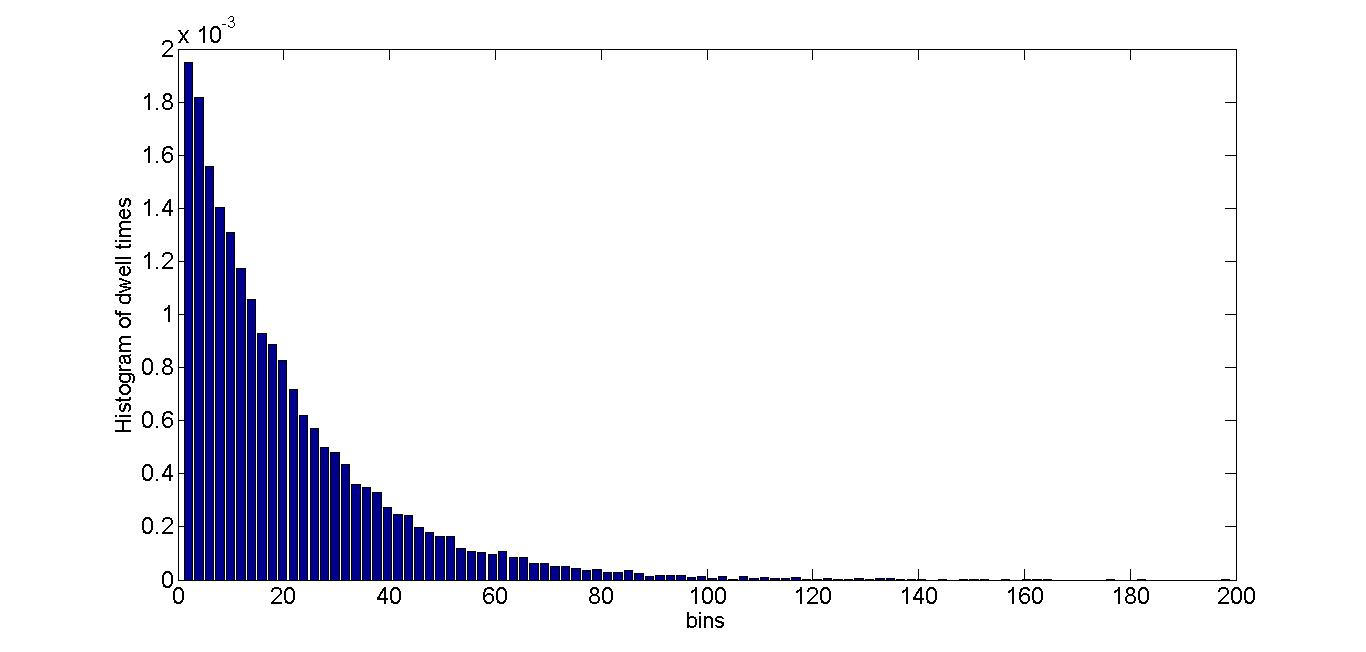
\includegraphics[width=12cm]{hist}
 	 	\caption{The histogram of dwell times}
 	 \end{figure}
 	 
   \begin{figure}[H]
   	\centering
   	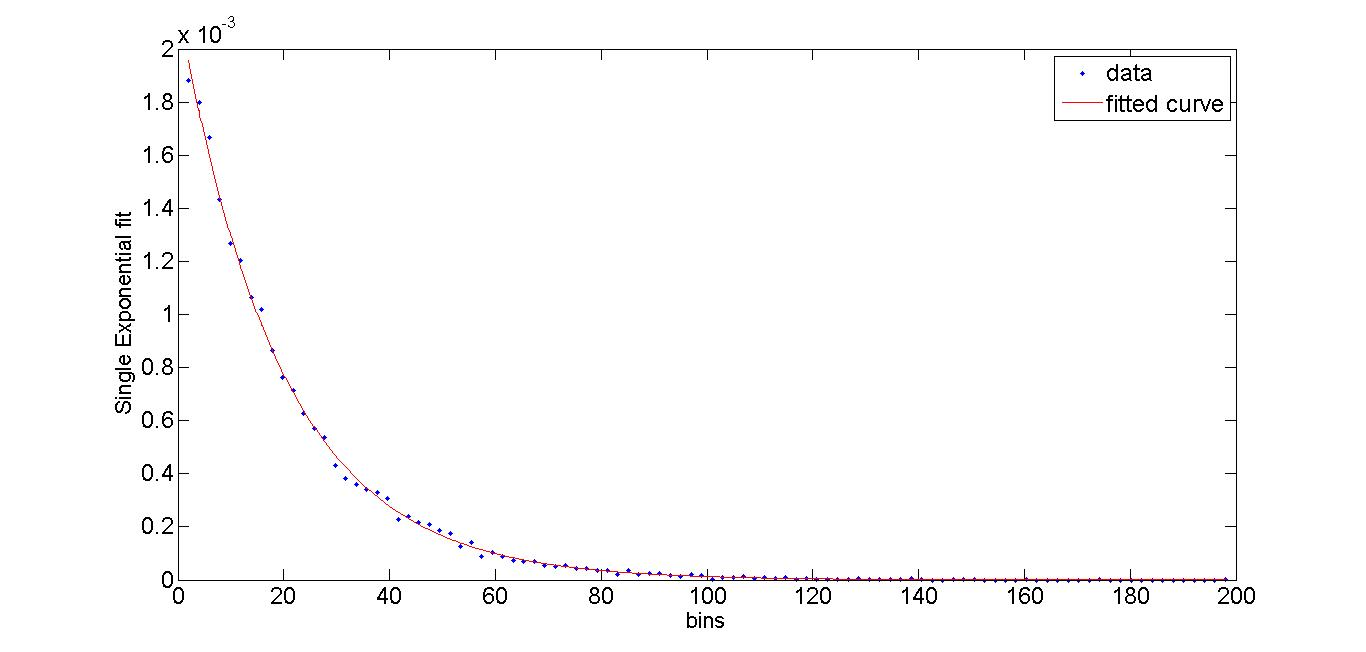
\includegraphics[width=12cm]{expfit}
   	\caption{The single exponential fit to the histogram}
   \end{figure}
   
   \begin{figure}[H]
   	\centering
   	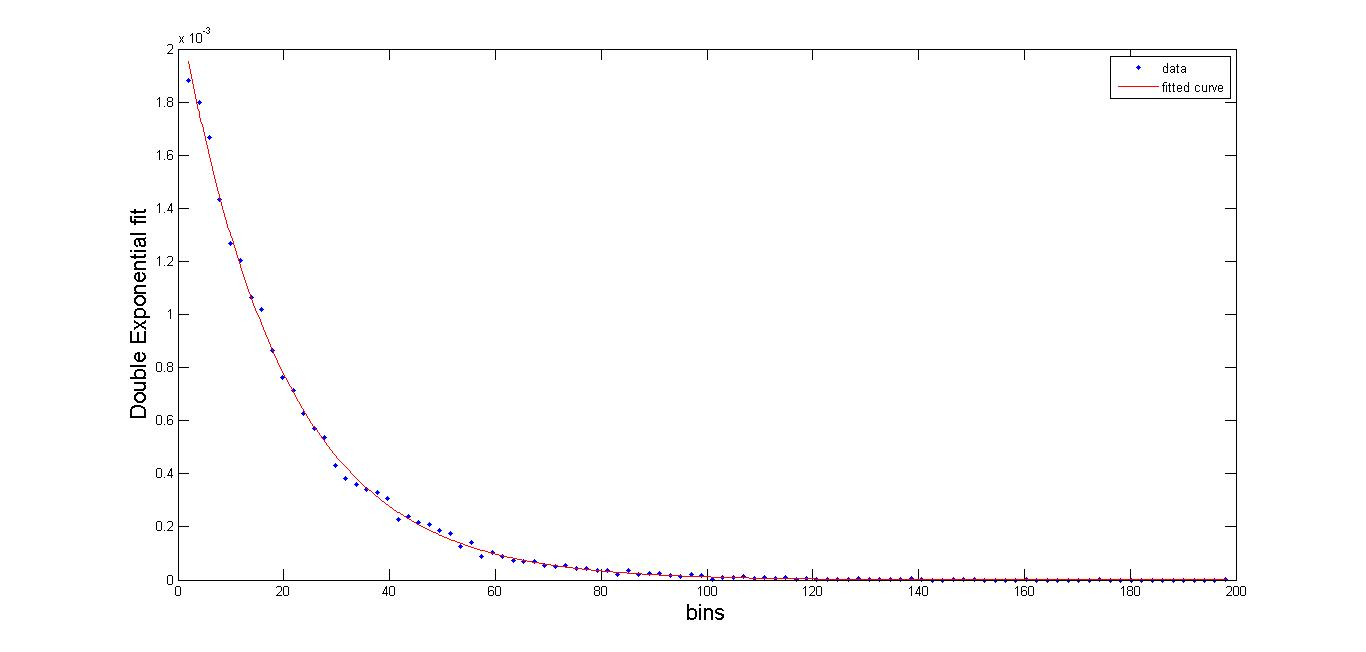
\includegraphics[width=12cm]{expfit2}
   	\caption{The double exponential fit to the histogram}
   \end{figure}   
   Obviously, the single exponential function is not a good fit because there are two eigenvalues for the system staying in the closed state.
 	  	 
 \end{itemize}



\section{Neural Spiking}

 	\begin{lstlisting}[language=Matlab,frame=single]
    %% Neural Spiking
    
    clear all;
    parpool; % Parallel computing because this takes a while
    
    A = [0.98, 0.1,0 ;
    0.02, 0.7,0.05;
    0 , 0.2, 0.95;] ;
    
    [T,L] =eigs(A);
    prb =T(:,1);
    probin =[prb(1)+prb(2);prb(3);];
    probin =probin./sum(probin);
    
    B = [0.9 0.1 0; 0.1 0.6 0.1; 0 0.3 0.9;];
    
    [T,L] =eigs(B);
    prb =T(:,1);
    probout =[prb(1)+prb(2);prb(3);];
    probout =probout./sum(probout);
    
    Popenout= 0.4;
    Popenin=0.6;
    Nin = 100;
    Nout =50;
    parfor T=0:1:Nin-1
	    sum=0;
	    for w = 0:1:Nout
		    sum=sum+ binopdf(w, Nout,Popenin)*(1-binocdf(T+w, Nin,Popenout));
		    if T+w>Nin
			    break;
		    end
	    end
	    p(T+1) =sum;
    end
    Nin = 10;
    Nout =5;
    parfor T=0:1:Nin-1
	    sum=0;
	    for w = 0:1:Nout
		    sum=sum+ binopdf(w, Nout,Popenin)*(1-binocdf(T+w, Nin,Popenout));
		    if T+w>Nin
			    break;
		    end
	    end
	    p2(T+1) =sum;
    end
    
    Nin = 1000;
    Nout =500;
    parfor T=0:1:Nin-1
	    sum=0;
	    for w = 0:1:Nout
		    sum=sum+ binopdf(w, Nout,Popenin)*(1-binocdf(T+w, Nin,Popenout));
		    if T+w>Nin
			    break;
		    end
	    end
	    p3(T+1) =sum;
    end
 	
 	\end{lstlisting}

   \begin{figure}[h]
   	\centering
   	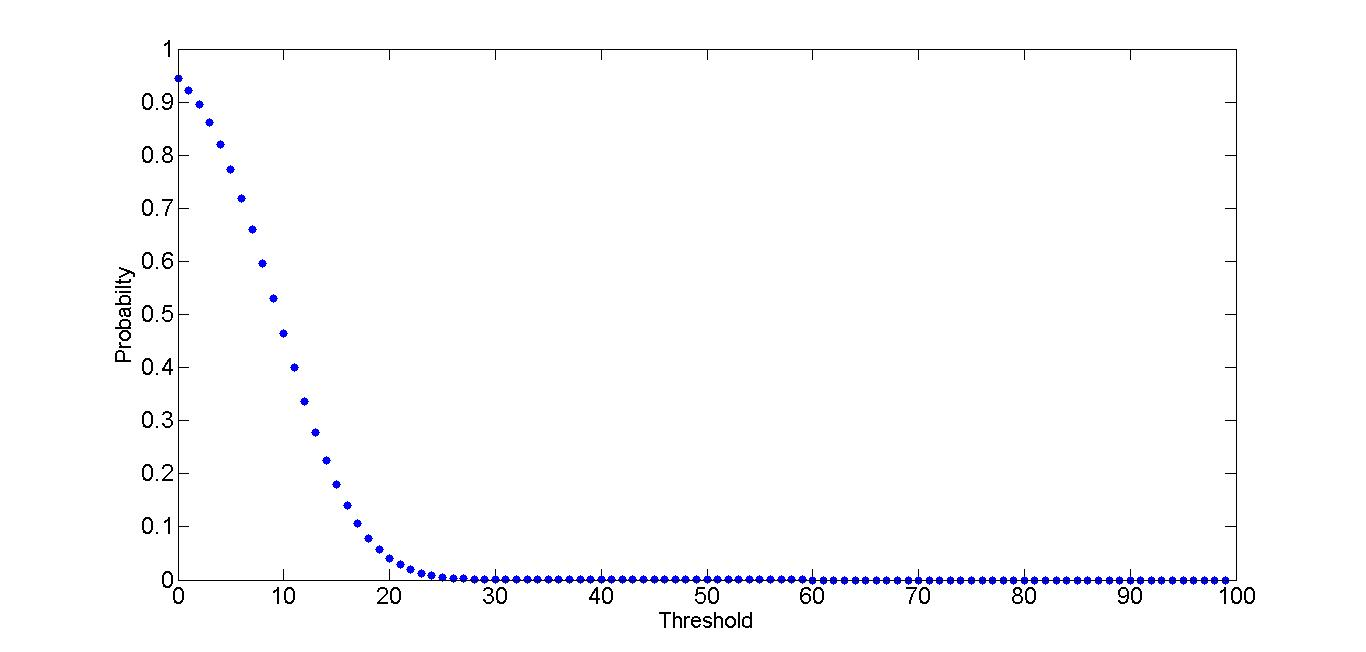
\includegraphics[width=12cm]{p1}
   	\caption{Distribution with $N_{inward}=100$ and $N_{outward}=50$}
   \end{figure}

   \begin{figure}[h]
   	\centering
   	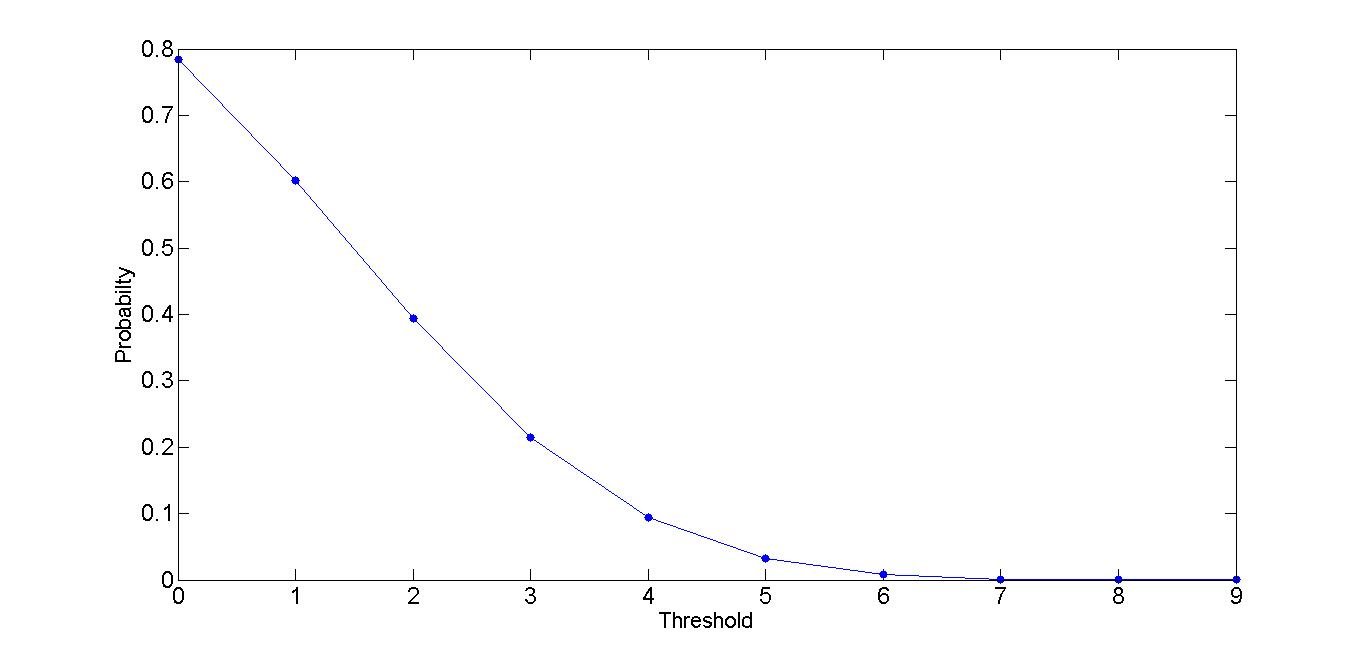
\includegraphics[width=12cm]{p2}
   	\caption{Distribution with $N_{inward}=10$ and $N_{outward}=5$}
   \end{figure}
   
   \begin{figure}[H]
   	\centering
   	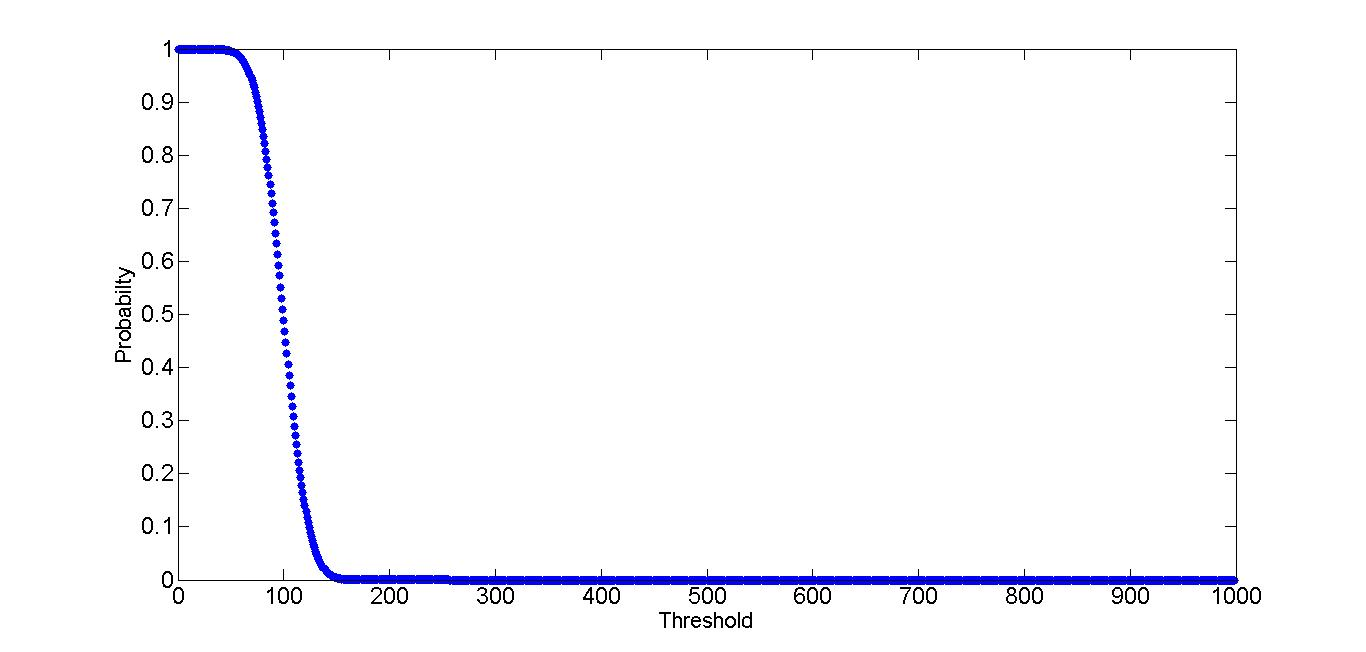
\includegraphics[width=12cm]{p3}
   	\caption{Distribution with $N_{inward}=1000$ and $N_{outward}=500$}
   \end{figure}  
   As we increase the number of channels, the distribution begins to look more and more like a guassian distribution, a good representation of the coin flipping.
       
\end{document}